% Minimal TikZ standalone example
\documentclass[tikz, border=1mm]{standalone}

\usepackage{amsmath}
\usepackage{tikz}

\usetikzlibrary{calc,angles,quotes}

\begin{document}

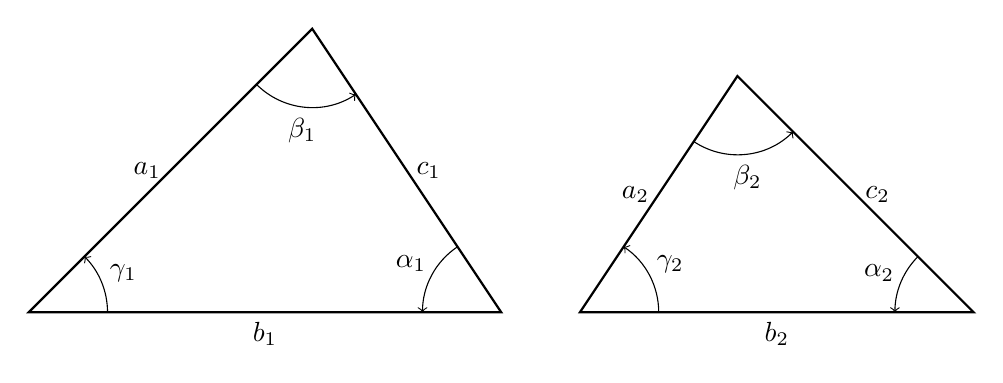
\begin{tikzpicture}[scale=1.0]
	% points
	\coordinate (A1) at (0,0);
	\coordinate (C1) at (6,0);
	\coordinate (B1) at ({18/5},{18/5});

	\coordinate (A2) at (7,0);
	\coordinate (C2) at (12,0);
	\coordinate (B2) at (9,3);

	% triangles sides
	\draw[thick] (A1) -- (B1) -- (C1) -- cycle;

	\draw[thick] (A2) -- (B2) -- (C2) -- cycle;

	% side labels
	\node[left]  at ($(A1)!0.5!(B1)$) {$a_1$};
	\node[below] at ($(A1)!0.5!(C1)$) {$b_1$};
	\node[right] at ($(B1)!0.5!(C1)$) {$c_1$};

	\node[left]  at ($(A2)!0.5!(B2)$) {$a_2$};
	\node[below] at ($(A2)!0.5!(C2)$) {$b_2$};
	\node[right] at ($(B2)!0.5!(C2)$) {$c_2$};

	% angles
	\pic[draw, ->, "$\alpha_1$", angle eccentricity=1.3, angle radius=1cm]
	{angle = B1--C1--A1};
	\pic[draw, ->, "$\beta_1$", angle eccentricity=1.3, angle radius=1cm]
	{angle = A1--B1--C1};
	\pic[draw, ->, "$\gamma_1$", angle eccentricity=1.3, angle radius=1cm]
	{angle = C1--A1--B1};

	\pic[draw, ->, "$\alpha_2$", angle eccentricity=1.3, angle radius=1cm]
	{angle = B2--C2--A2};
	\pic[draw, ->, "$\beta_2$", angle eccentricity=1.3, angle radius=1cm]
	{angle = A2--B2--C2};
	\pic[draw, ->, "$\gamma_2$", angle eccentricity=1.3, angle radius=1cm]
	{angle = C2--A2--B2};

\end{tikzpicture}

\end{document}
